\chapter{Evaluation}
This chapter presents and describes the results gathered in the final test. The results from both the Overloaded and Intermixed version is presented and compared with visual representations.

\section{Final test}
The final test was done on Aalborg Unitversity Campus in the Multi Sensory Lab's Anechoic chamber. The chamber was used was to reduce the amount of outside distractions and noises which could potentially be in the lab. The test was done using simple random sampling, and a semi structured interview as explained in \autoref{methods:ft}. The test was conducted on 20 people (10 for each version of the prototype) aged 21-45. The participants would besides the questions listed in appendix \ref{FinalTestQuestions}, also asked about their enjoyment and their engagement in using the prototype.
    
\subsection{Test setup}
    The final test setup included an observer which acted as a note taker and a moderator, that maintained the flow of the test, and conducted the interview, in addition to answering any questions the test participant had. As seen in figure \autoref{fig:final_test_setup} the participant would be seated where the HMD was located next to the moderator. The participant would first go through a short demographics survey, and then led into the anechoic chamber which is completely soundproof. This helps the participants' immersion while also reducing outside distractions.
    
    \begin{figure}[H]
        \centering
        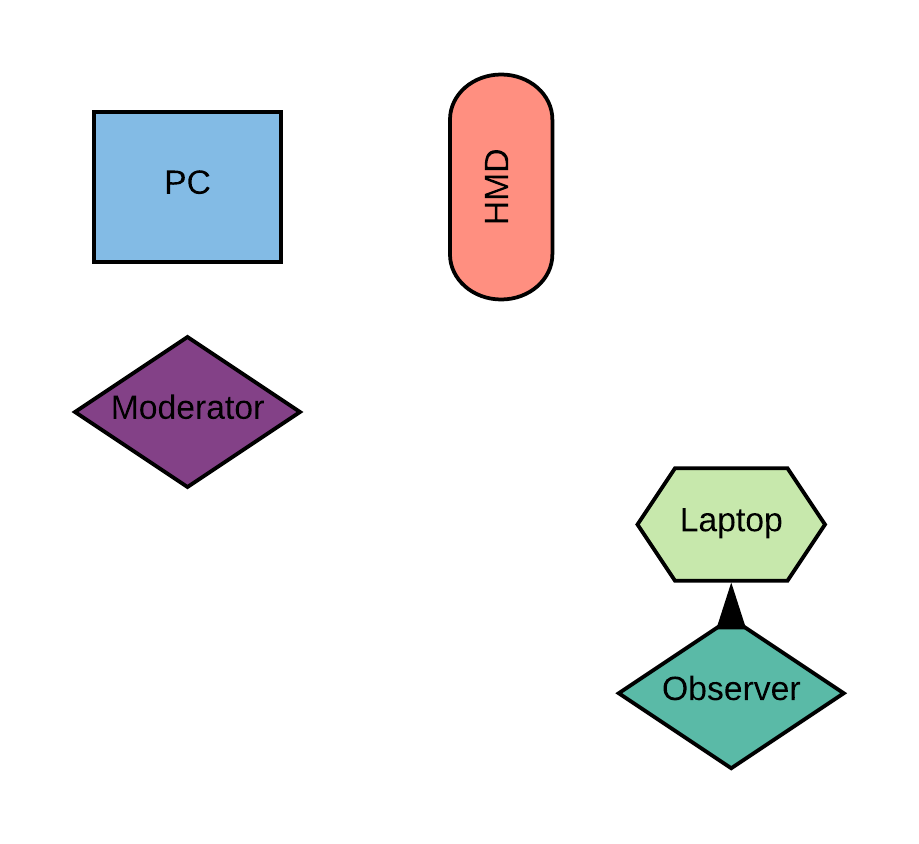
\includegraphics[width=0.6\linewidth]{figure/Evaluation/FinalTestSetup.png}
        \caption{Figure showing the final test setup.}
        \label{fig:final_test_setup}
    \end{figure}
    
\section{Test results}
This section will present the results gathered from the interviews. The results have been coded and analysed using traditional coding \cite{bjoernerBog}. In \autoref{fig:IntermixedEnjoyEngage} and \autoref{fig:OverloadEnjoyEngage} The results from both prototypes can be seen. Each prototype version had 10 participants answer on a scale from 1-7 where 4 is neutral, how engaged and how much they enjoyed using the prototype. In \autoref{fig:IntermixedEnjoyEngage} the intermixed prototype's results show that the mean of the rated enjoyment is 4.5 which is on the positive side of the scale. Similarly, in  \autoref{fig:OverloadEnjoyEngage} the overloaded prototype's enjoyment mean is 5.1 which is higher than the intermixed versions enjoyment. Both versions' engagement tested the exact same engagement which is equal to 4.6 which is also on the positive side on the scale.

    \begin{figure}[H]
        \centering
        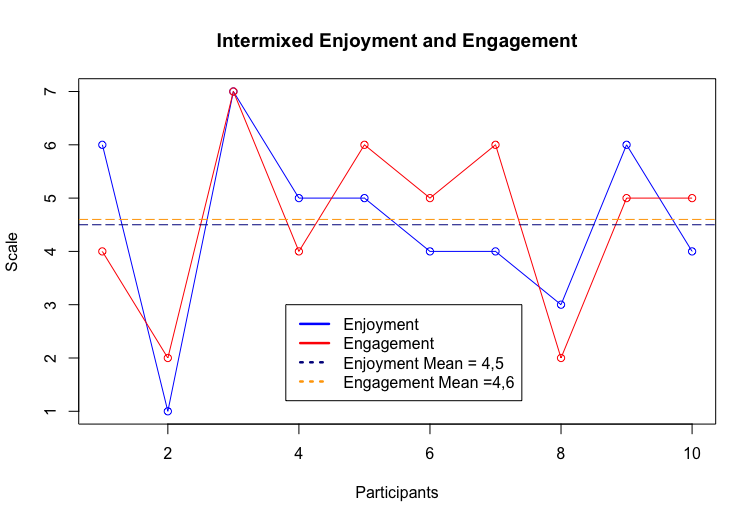
\includegraphics[width=0.99\linewidth]{figure/Evaluation/IEnjoy.png}
        \caption{Plot of intermixed enjoyment and engagement.}
        \label{fig:IntermixedEnjoyEngage}
    \end{figure}
    \begin{figure}[H]
        \centering
        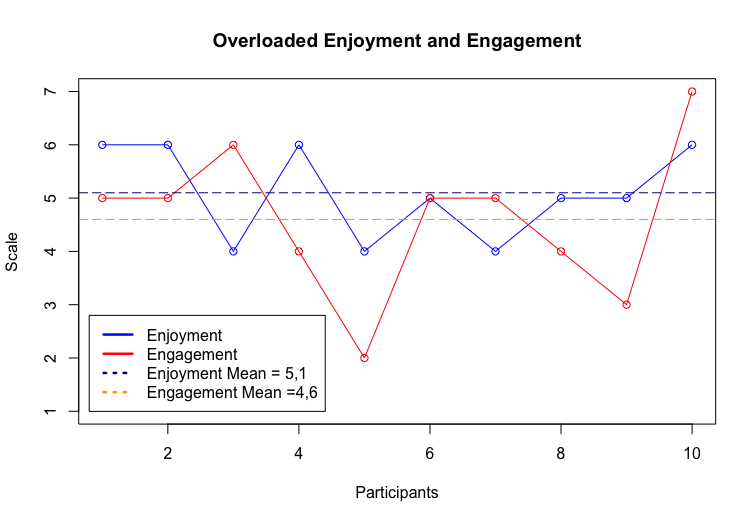
\includegraphics[width=0.99\linewidth]{figure/Evaluation/OEnjoy.png}
        \caption{Plot of overloaded enjoyment and engagement.}
        \label{fig:OverloadEnjoyEngage}
    \end{figure}

After using the prototype the participants were asked a list of questions following the semi-structured interview form which means that the ordering of the topics can vary depending on the respondents answers. In figure \autoref{fig:EvalCoding} the key points from the interview is coded into boxes. The major themes and view points expressed by the participants a color coded and drawn together with sources.

On the left side colored with green and dark green is major-themes and in light green is sub themes and sources. One major theme is the message of the game, the participants were asked if they understood the message of the game after trying the experience. The intermixed version showed that more people pointed to the message being related to climate change, while the overloaded version was more apparent and the participants said meat consumption was the message. 

In correlation to the message, the participants were also asked about the radio and the purpose of it. In the intermixed version participants expressed that they misunderstood the purpose of the radio, however, they did catch on to the radio messages were related to the environment and climate change. In the overloaded version, the messages were more frequent and the majority of the participants caught onto that the radio was talking about meat consumption. 

A last major theme was the respondents were asked if they felt like eating less burgers during the experience. This was to see if the participants where more aware of their actions after catching on to the message of the game. In the intermixed version, none of the participants felt like eating less burgers during the experience, and it was expressed that the burger was the only interaction element. In the overloaded version, a few of the respondents felt like eating less burgers when they noticed the environment changing and when they heard some of the messages from the radio.

Next to the major themes, the participants were also asked about their view on the message of the game and their view on meat consumption after trying the experience. In neither the overloaded nor the intermixed version any of the participants clearly stated that the message came on too strong. In the intermixed version, half of the asked respondents had a positive view on meat consumption, and would consider eating less meat after trying the game. They expressed that the radio and the environment were key factors to their view change. On the opposite side, the negative respondents expressed that they already cut down on meat consumption or they were vegan or vegetarian. In the overloaded version only 1 out of the 10 asked participants would consider eating less meat after trying the experience, this was also due to the effects seen on the environment in the game. On the negative side, the participants expressed that they already have a firm standpoint on meat consumption, or the burger in the game was not convincing enough for them to cut down.

        \begin{figure}[H]
        \centering
        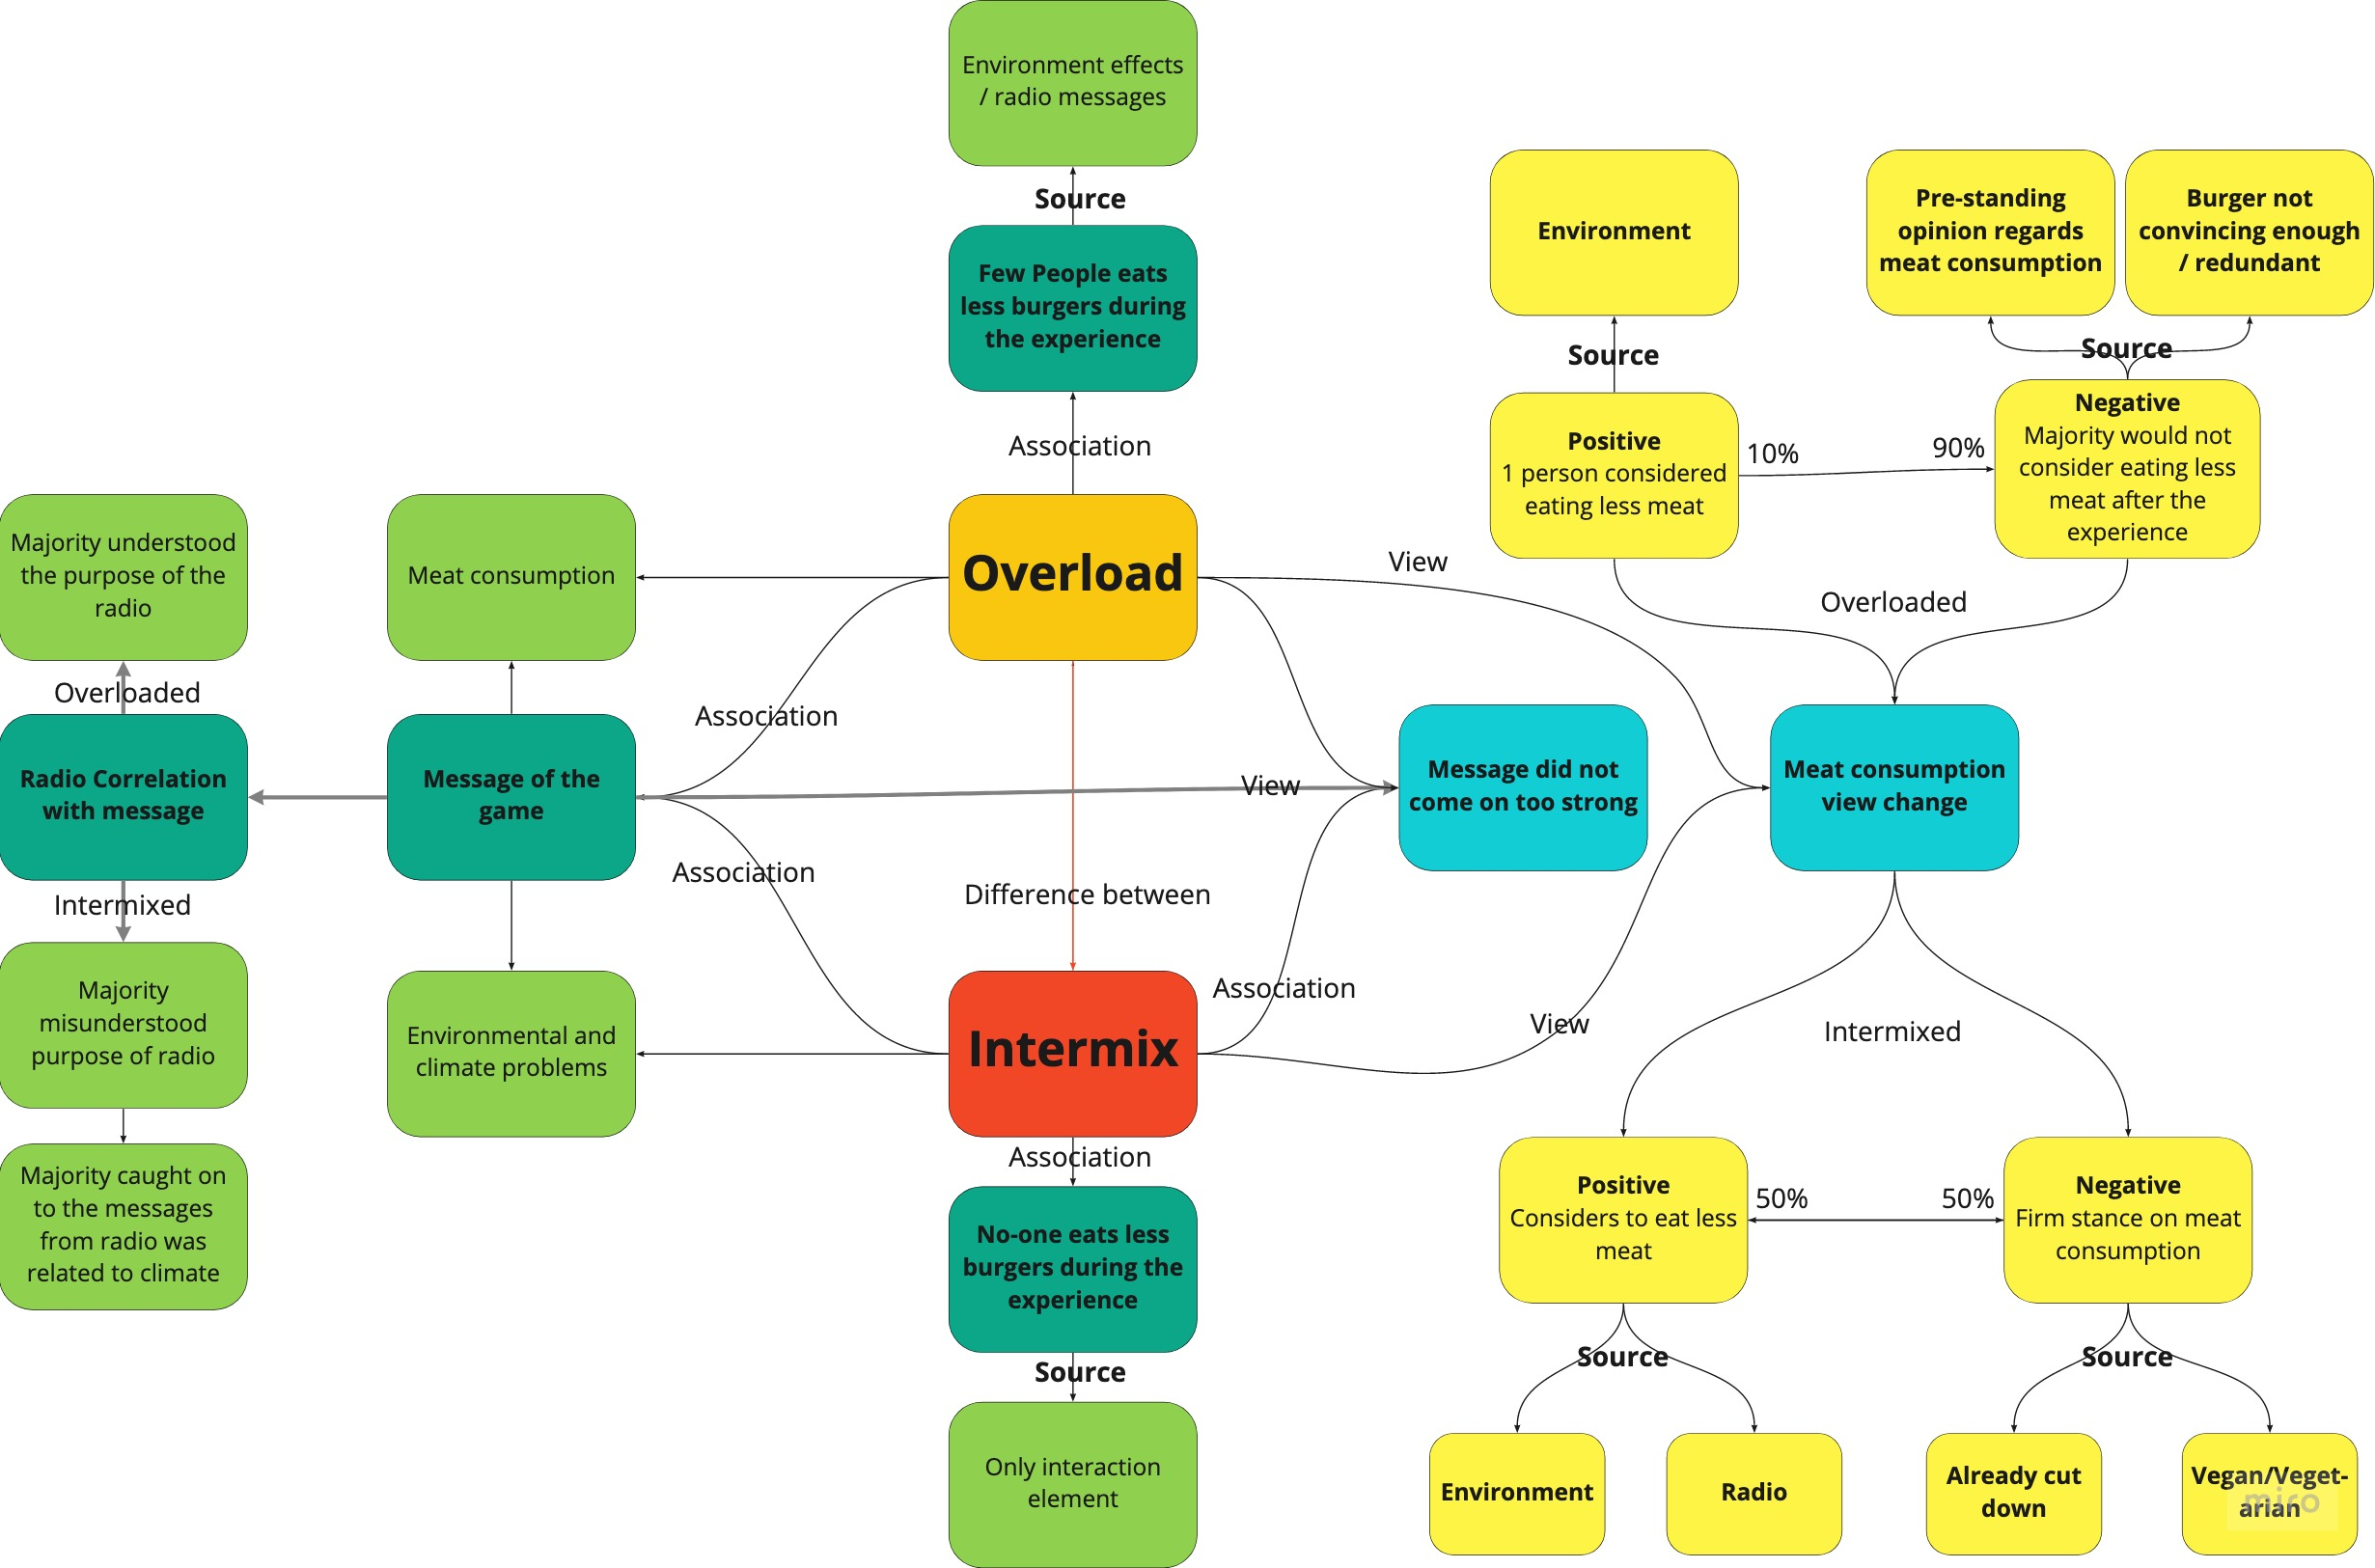
\includegraphics[width=1\linewidth]{figure/Evaluation/eval.jpg}
        \caption{Coding of interview results.}
        \label{fig:EvalCoding}
    \end{figure}
    
\section{Summary}
In regards to enjoyment and engagement, the overloaded version had a a 0.6 higher average enjoyment over the intermixed version. However, both versions had the exact same engagement mean of 4.6.

The main difference between the intermixed and the overloaded version is the respondents view on meat change after trying the game. The intermixed version had more success in convincing more respondents to consider eating less meat than the overloaded version. It was also apparent that neither of the versions' message came on too strong. 